\documentclass{beamer}
\usetheme{}
\usecolortheme{dolphin}           
\useinnertheme{circles}
\setbeamertemplate{itemize items}[default]
\setbeamertemplate{enumerate items}[default]
\usepackage[T1]{fontenc}
\usepackage[utf8]{inputenc}
\usepackage{lmodern}
\usepackage{amsmath}
\usepackage{booktabs} 
\usepackage{graphicx}        
\usepackage{array}
\usepackage{color}
\makeatletter
\def\zapcolorreset{\let\reset@color\relax\ignorespaces}
\def\colorrows#1{\noalign{\aftergroup\zapcolorreset#1}\ignorespaces}
\makeatother
\graphicspath{{/home/swl/Dropbox/ucd/advanced_macro/figures/}} 
\setbeamertemplate{navigation symbols}{}
\setbeamertemplate{footline}[frame number]

%--------------------------------------
\title{Lending}
\author{School of Economics, University College Dublin}
\date{Spring 2018}
\begin{document}

%--------------------------------------
\begin{frame}
 \titlepage
\end{frame}
%--------------------------------------

%--------------------------------------
\begin{frame}
 Recall interest rate equation from NK model
  \begin{align} 
  i_t=r_t^n+ \phi_{\pi}\pi_t+\phi_xx_t 
\end{align}
\medskip
$i_t$ is a specific interest rate
\begin{itemize}
  \item Short-term risk-free overnight rate that banks charge each other
  \item Quite different from consumer interest rates
\end{itemize}
\medskip
To understand consumer interest rates need to understand risk involved with consumer lending. 
\end{frame}
%--------------------------------------

%--------------------------------------
\begin{frame}
 Suppose investor can choose between following two assets  
\begin{enumerate}
  \item Risk-free bond with interest rate $r$
  \item Loan with interest rate $R$ and probability of default $p$
  \begin{itemize}
    \item Return of $R$ with probability $1-p$
    \item Return of -1 (losing all your money) with probability $p$
  \end{itemize}
\end{enumerate}
\end{frame}
%--------------------------------------

%--------------------------------------
\begin{frame}
  Expected return on loan
  \begin{align}
    R-Rp-p\\ \nonumber
    R-p
\end{align}
 For same expected return, interest rate needs to be
\begin{align}
  R-p=r\\ \nonumber
  R=r+p
\end{align}
\end{frame}
%--------------------------------------

%--------------------------------------
\begin{frame}
 If loan comes with collateral, default implies return
\begin{align}
  c-1<0  
\end{align}
We get
\begin{align}
  R=r+(1-c)p  
\end{align}
 \medskip
 This entails that
 \begin{enumerate}
   \item Collateralised loans have lower interest rates
   \item Interest rate depends on type of collateral
 \end{enumerate}
\end{frame}
%--------------------------------------

%--------------------------------------
\begin{frame}
  \begin{figure}
    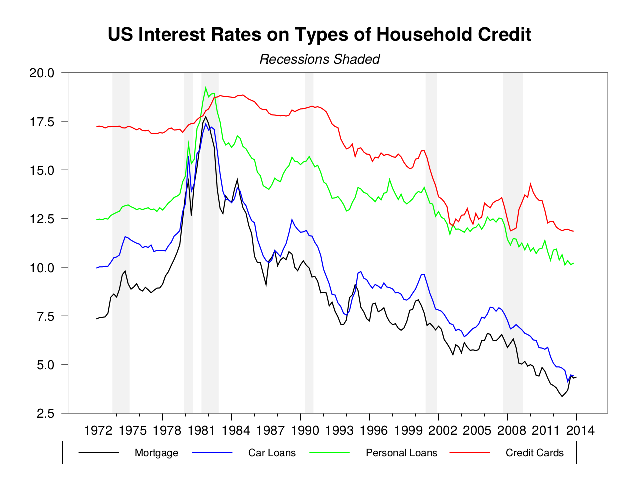
\includegraphics{us_interest_rates.eps}
  \end{figure}
\end{frame}
%--------------------------------------

%--------------------------------------
\begin{frame}
  \begin{figure}
    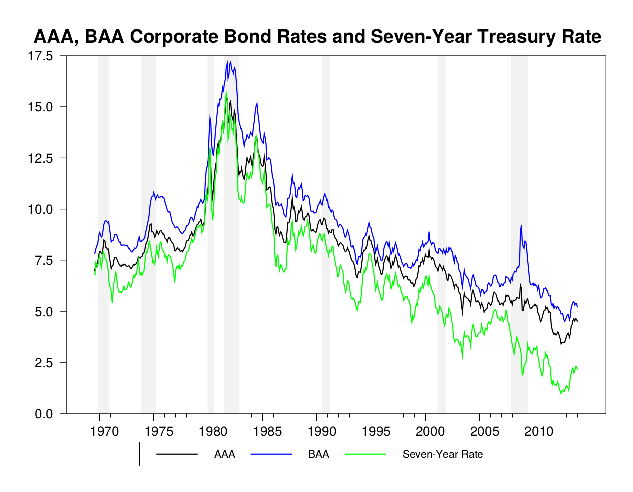
\includegraphics{bond_rates.eps}
  \end{figure}
\end{frame}
%--------------------------------------

%--------------------------------------
\begin{frame}
 Concerning default risk and collateral 
\begin{enumerate}
  \item Interest rate is affected by the value of the collateral
  \item Value of assets fluctuate with the state of the economy
\end{enumerate}
 \medskip
 Suggests mechanism by which financial sector can propagate business cycle shocks: \textbf{financial accelerator}
 \begin{itemize}
   \item shock that produces a recession will lead to higher interest rate spreads for borrowers which will worsen the recession. 
 \end{itemize}
\end{frame}
%--------------------------------------

%--------------------------------------
\begin{frame}
Bernanke \& Gertler (1989) \\
  Aggregated demand is given by
\begin{align}
  y_t &= \frac{C}{Y}c_t + \frac{I}{Y}inv_t + \frac{G}{Y}g_t + \frac{C^e}{Y}c^e_t+...\\
  c_t &= -\sigma r_{t+1} + E_tc_{t+1}\\
  c^e_t &= \frac{1-\phi}{\phi}n_{t+1}\\
  q_t &= \phi(i_t-k_t)  \\
  E_tr_{kt+1} &= (1-\rho)E_t(p_{wt+1}-p_{t-1} + y_{t-1} - k_{t+1}) + \rho E_tq_{t+1} -q_t\\
  E_tr_{kt+1} - r_{t+1} &= -v(n_t -q_t -k_{t+1})  
\end{align}
\end{frame}
%--------------------------------------

%--------------------------------------
\begin{frame}
  And aggregate supply is given by
\begin{align}
  y_t &= a_t + \alpha k_t + (1-\alpha)l_t\\
  y_t-l_t &= \mu_t + \gamma_l l_t + c_t\\
  \pi_t &= \kappa (p_{wt}-p_t) + \beta E_t \pi_{t+1}
\end{align}
\end{frame}
%--------------------------------------

%--------------------------------------
\begin{frame}
  The evolution of the state variable is described by
\begin{align}
  k_{t+1} &= \delta inv_t + (1-\delta)k_t\\
  n_t &= \frac{\theta RK}{N}[r_ t^k - r_t] + \theta R(r_t+n_{t-1})\\
  r_t &= i_{t-1} - \pi_{t-1}
\end{align}
\end{frame}
%--------------------------------------

%--------------------------------------
\begin{frame}
  And finally the monetary policy rule is given by
\begin{align}
  i_t &= \rho i_{t-1} + (1-\rho)[\gamma_{\pi}\pi_t + \gamma_y(y_t - y_t^n)]+ \epsilon_t^{rn}\\
  i_t &= r_{t+1} - E_t\pi_{t+1}
\end{align}
\end{frame}
%--------------------------------------

%--------------------------------------
\begin{frame}
Borrowers with higher risk pay higher interest rates.
\begin{itemize}
  \item Assumption: for each risk level, someone willing to lend at high enough rates
  \item Credit suppliers can refuse to make a loan, rather than trying to balance the loss by raising the interest rate. 
\end{itemize}
\medskip
This is called \textbf{credit rationing}
\begin{quote}
  Lenders provide a smaller amount of loans than is demanded at the market interest rate.
\end{quote}
\end{frame}
%--------------------------------------

%--------------------------------------
\begin{frame}
 Credit rationing can be quite severe, turning down credit-worthy borrowers
The problem here is that there is asymmetric information due to the fact that 
\begin{itemize}
  \item Banks can't always tell good borrowers from bad
  \item From bank's point of view borrowers worsen as interest rates increase
\end{itemize}
  \medskip
  Issue of information asymmetry
\end{frame}
%--------------------------------------

%--------------------------------------
\begin{frame}
 \textbf{Stiglitz \& Weiss} (1981); Suppose number of borrowers each with a project to undertake
\begin{enumerate}
  \item All borrowers look to borrow $B$ and put up collateral $C$
  \item Projects deliver a sum of $R$  
  \item Interest rate on bank loans $r$ is determined endogenously
\end{enumerate}
\end{frame}
%--------------------------------------

%--------------------------------------
\begin{frame} 
 Return $R$ is uncertain
 \begin{itemize}
   \item Outcome distribution varies across borrowers 
 \end{itemize}
 \medskip
 Return distribution type $\theta$ borrowers 
 \begin{align}
   f(R,\theta)
 \end{align}
 \medskip
 Distribution mean identical across borrowers, but greater $\theta$ values correspond to greater riskiness
 \begin{itemize}
   \item High values of $\theta$ induce a mean-preserving spread in the distribution of projected payoffs
   \item Borrowers are observably identical to banks: don't observe an individual's value of $\theta$
 \end{itemize}
\end{frame}
%--------------------------------------

%--------------------------------------
\begin{frame}
 Mechanism: bank sets $r$ which might affect risk of loan through
\begin{enumerate}
  \item \textbf{Adverse selection}: Sorting potential borrowers
  \item \textbf{Moral hazard}: Affecting the actions of the borrowers
\end{enumerate}
\end{frame}
%--------------------------------------

%--------------------------------------
\begin{frame}
 Default occurs when
\begin{align}
  C+R\leq B(1+r)
\end{align}
\medskip
where $B$ being the amount borrowed, and $C$ the collateral.\\
Return to firm $\pi(R,r)$ given by
\begin{align}
  \pi(R,r)=Max(R-(1+r)B;-C)
\end{align}
\medskip
Return to the bank can be written as 
\begin{align}
  \rho(R,r)=min(R+C;B(1+r))
\end{align}
\end{frame}
%--------------------------------------

%--------------------------------------
\begin{frame}
The worst a firm can do is default on the loan and lose the collateral when the project has a bad return
\begin{itemize}
  \item After that the return increases one for one with outcome $R$
  \item Return depends negatively on borrowing rate $r$
  \item Not all firms decide to go ahead and borrow as not all firms have a positive expected value.
\end{itemize}
\end{frame}
%--------------------------------------

%--------------------------------------
\begin{frame}
Firm borrows if
\begin{align}
  \mathbb{E}[\pi(R,r)]=\int_0^{\infty} \pi(R,r)f(R,\theta)dR>0
\end{align}
\medskip
Main question is how 
\begin{align}
  \mathbb{E}[\pi(R,r)]
\end{align}
\medskip
varies with type $\theta$
\end{frame}
%--------------------------------------

%--------------------------------------
\begin{frame}
\textbf{Borrower pool}: Decide to borrow if
\begin{align}
  \theta > \hat{\theta}(r)
\end{align}
\medskip
From utility theory;
\begin{itemize}
  \item If $U(C)$ is concave: mean-preserving spread in $C$ distribution reduces expected utility because people are risk averse
\end{itemize}
\medskip
In this case outcome is a convex function of $R$, so more uncertainty increases the expected return. 
\begin{itemize}
  \item Bad case:outcome still $−C$ but increased risk raises the chance of a really good outcome.
\end{itemize}
\end{frame}
%--------------------------------------

%--------------------------------------
\begin{frame}
 How does $r$ increase affect loan demand?  
\begin{itemize}
  \item Project returns depend negatively on $r$: increase in $r$ reduces everyone's expected project returns  
  \item Expected project returns depend positively on $\theta$: some firms still have positive expected value for
    going ahead with borrowing and doing the project
  \item Increase in $r$ raises the cut-off $\hat{\theta}(r)$ for potential borrowers
\end{itemize}
\medskip
 Interest rate increases; borrowers pool changes consisting of more risky project (adverse selection)
 \begin{itemize}
   \item Moral hazard problem: risk-neutral investors prefer project with higher bankruptcy probability
 \end{itemize}
\end{frame}
%--------------------------------------

%--------------------------------------
\begin{frame}
Bank pay off given by
\begin{align}
  Min(R+C;(1+r)B)
\end{align}
 If bank knows it is lending to type $\theta$; expected return
\begin{align}
  \rho(\theta,r)=\int_0^{\infty}[Min(R+C;(1+r)B)]f(R,\theta)dR
\end{align}
 \medskip
 Bank's pay off concave function of $R$: increases in $\theta$ reduces bank's expected return.
\end{frame}
%--------------------------------------

%--------------------------------------
\begin{frame}
 \begin{enumerate}
   \item Best case: bank gets principal and interest
   \item Worst case: only get collateral
 \end{enumerate}
 \medskip
 More risk is bad, but bank cannot tell if borrowers is risky
 \begin{itemize}
   \item Expected payoff can be calculated averaging across all types that look for loans at interest rate $r$
 \end{itemize}
\begin{align}
  \mathbb{E}[\rho(\theta,r)]=\frac{\int_{\hat{\theta}(r)}^{\infty}\rho(\theta,r)dG(\theta)}{1-G(\hat{\theta})}
\end{align}
\end{frame}
%--------------------------------------

%--------------------------------------
\begin{frame}
 $r$ increase has two effects on bank's pay off 
\begin{enumerate}
  \item +ve: higher interest revenues from each project that pays off
  \item -ve: adverse selection.   
\end{enumerate}
At some point second effect dominates: bank profits rise as the interest rate goes up, reach a maximum and then decline
\end{frame}
%--------------------------------------

%--------------------------------------
\begin{frame} 
  Assume there are only two types of borrowers, low and high risk. 
Profits drop at the point where the low-risk types drop out.
Extended to a continuous number of types, this implies a particular interest rate $r^*$, which is consistent with a maximum level of profits.
We assume that loan supply depends positively on the expected pay off. Note however, that banks can't simply choose the interest rate $r^*$, simply because they'd like this outcome. If there isn't sufficient demand to meet this supply, then this can't be an equilibrium: Banks would be chasing customers offering them $r^*$ and lots of people would be turning them down.
\end{frame}
%--------------------------------------

%--------------------------------------
\begin{frame}
 Equilibrium outcome determined by supply/demand interaction
\begin{enumerate}
  \item Low loan demand
  \begin{itemize}
    \item Loan demand curve intersects loan supply curve below $r^*$. 
    \item Market functions normally: all who request a loan receive one
\end{itemize}
  \item High loan demand
  \begin{itemize}
    \item Loan demand and supply curves do not intersect: bank pick optimal interest rate $r^*$    
    \item Credit rationing: More demand than banks are willing to supply
  \end{itemize}
\end{enumerate}
\end{frame}
%--------------------------------------

%--------------------------------------
\begin{frame}
 Sovereign defaults (textit{incomplete list}):\\
 \medskip
 Early 1800s: number of countries after the Napoleonic Wars, e.g. Denmark, France, the Netherlands, and Sweden\\
 1875: Ottoman Empire\\
 1932: Germany\\
 1982: Mexico\\
 1998: Russia\\
 2006: Zimbabwe\\
 1982, 1989, 2001: Argentina\\
 1826, 1843, 1860, 1894, 1932, 2015: Greece
\end{frame}
%--------------------------------------

%--------------------------------------
\begin{frame}
figure 
\end{frame}
%--------------------------------------

%--------------------------------------
\begin{frame}
  Consider country has $P(default)=0.1$ over next year; leading to 50\% default on outstanding debt
  \begin{itemize}
    \item Country needs to pay 5\% premium on debt relative to safe assets
  \end{itemize}
  \medskip
  Premium imposes additional burden on government
  \begin{itemize}
    \item Interest costs rise above the funds that country can access to pay off the interest payments
    \item Alternatively the country's GDP could expand in order to keep debt stable
  \end{itemize}
  Market for government bonds might cease to operate as the country is deemed not credit-worthy: risk goes from unlikely to likely
  \begin{itemize}
    \item Closing of a bond market is an rare and abrupt events: People often don't see it coming
  \end{itemize}
  After a default a country needs to restructure it debt which often involves writing off part of it, in order to restore the debt level to a more sustainable level. 
\end{frame}
%--------------------------------------

%--------------------------------------
\begin{frame}
 Two types of banking relevant to today's financial system
\begin{enumerate}
  \item Clearing house banks
  \item Fractional reserve banking
\end{enumerate}
\end{frame}
%--------------------------------------

%--------------------------------------
\begin{frame}
 Why are financial intermediaries useful?
\begin{enumerate}
  \item Pooling savings  
  \item Risk diversification
  \item Maturity transformation
  \item Information processing  
\end{enumerate}
\end{frame}
%--------------------------------------

%--------------------------------------
\begin{frame}
  Suppose that one business day the following transactions occur
\begin{itemize}
  \item Bank A's depositors have accounts credited with EUR 10 million from Bank B's depositors
  \item Bank B's depositors will be credited with EUR 9 million from Bank A's depositors
\end{itemize}
 \medskip
 Total transfers: EUR 19 million\\
 \begin{enumerate}
   \item Have couriers transfer money back and forth
   \item Settle account at end of the business day
 \end{enumerate}
\end{frame}
%--------------------------------------

%--------------------------------------
\begin{frame}
  \textbf{Clearing house bank}
  \begin{itemize}
  \item Clearing house will order transfer of EUR 1 million from Bank B to Bank A
  \item More efficiently: Deduct EUR 1 million from ledger entry for Bank B's account,  add it to Bank A's
  \item All deposits still fully backed by the cash in the vaults
\end{itemize}
\medskip
Forerunner of today's central banks
\end{frame}
%--------------------------------------

%--------------------------------------
\begin{frame}
 Most of time only small small fraction of bank's total deposits will be demanded on any given time
 \begin{itemize}
   \item "most" being important qualifier here
 \end{itemize}
 i.e. not all cash has to be in the vault in order to back up the deposits
 \begin{itemize}
   \item Some of it can be used for loans while keeping some cash reserves to deal with day-today demand. 
 \end{itemize}
This practice is called \textbf{fractional reserve banking }
\end{frame}
%--------------------------------------

%--------------------------------------
\begin{frame}
 Some advantages of fractional reserve banking
\begin{enumerate}
  \item Saves depository money: banks can charge interest on loans
  \item Banks serve as an intermediary  
\end{enumerate}
\end{frame}
%--------------------------------------

%--------------------------------------
\begin{frame}
 Disadvantage of fractional reserve banking is risk of bank run  
\begin{itemize}
  \item Bank supposed to have assets greater than liabilities owed to non-investors(positive bank capital)
  \item It could be the case that the bank makes loans to borrowers who default
  \item When customers suspect that the bank does not have the assets to pay back money they might want to have their money back
  \item This could lead to a run on the bank: many depositors want their money back. 
  \item Many banks are unable to cope with bank runs
\end{itemize}
 \medskip
 Potential for instability due to maturity mismatch
 \begin{itemize}
   \item People who supply funds want to have it available for return at shorter terms than the people who the bank lends the money to
 \end{itemize}
\end{frame}
%--------------------------------------

%--------------------------------------
\begin{frame}
 Bank's balance sheet lists assets and liabilities  
\begin{itemize}
  \item Liabilities: sources of the bank's funds
  \item Assets: uses of said funds
\end{itemize}
\end{frame}
%--------------------------------------

%--------------------------------------
\begin{frame}
 Some risks of assets
\begin{itemize}
  \item Borrowers don't pay back loans
  \item Bad investments are sometimes made in stocks and bonds
  \item Other assets invested in lose much of their value
\end{itemize}
\medskip
 Might result in negative equity capital
 \begin{itemize}
   \item Assets go below what it owes to depositors and bond-holders
   \item Might trigger bank run when bank is suspected to be insolvent
 \end{itemize}  
\end{frame}
%--------------------------------------

%--------------------------------------
\begin{frame}
 Some recent bank runs\\
 \medskip
 2001: Bank run in Argentina during economic crisis (1999-2002)
 2007: Northern Rock, UK\\
 2009: DSB Bank, the Netherlands\\
 2015: Bank runs in Greece and Cyprus
\end{frame}
%--------------------------------------

%--------------------------------------
\begin{frame}
  Couple of things happen during a bank run 
\begin{enumerate}
  \item Banks starts paying off depositors; selling off most liquid assets: e.g. cash, excess reserves at central bank, etc.
  \item Bank sells non-liquid assets: long-term customer loans, property assets: fire sale
\end{enumerate}
 \medskip
 Bank runs often triggered by - assumed- insolvency of bank: makes make more insolvent
 \begin{itemize}
   \item Bank run can be triggered by just rumours
   \item Banks and governments are always quick to declare that the banks are fully solvent
   \item Main concern of bank run is contagion risk
 \end{itemize}
\end{frame}
%--------------------------------------

%--------------------------------------
\begin{frame}
\begin{table}[!h] \centering
\caption{Stylised bank balance sheet}
\scalebox{1}{
\begin{tabular}{ll}
\\[-1.8ex]\hline \hline \\[-1.8ex]
    Assets (use of funds)  & Liabilities (source of funds)\\
    \hline \\ 
    Loans & Deposits\\
    Securities & Other borrowings\\
    Cash and reserves  & Equity capital\\
    \\[-1.8ex]\hline \hline \\[-1.8ex]
    \end{tabular}}
\end{table}
\end{frame}
%--------------------------------------

%--------------------------------------
\begin{frame}  
Banking crisis likely leads to credit squeeze
\begin{align*}
  Loans= Deposits + Other\;Borrowings + Equity\;Capital\\
  - Cash\;and\;reserves -   Securities
\end{align*}
\end{frame}
%--------------------------------------

%--------------------------------------
\begin{frame}
  \begin{enumerate}
  \item Loans
  \begin{itemize}
    \item Hard for bank to call in loans
    \item When loan is paid off, bank will keep funds as cash, reserves, or invest in securities
    \item Or pay off deposit outflows or maturing bond liabilities
    \item Don't make new loans
  \end{itemize}
  \item Deposits
  \begin{itemize}
    \item Customers prefer to keep cash at home
    \item Banks will have less funds to loan
  \end{itemize}
  \item Other borrowings
  \begin{itemize}
    \item Bond markets/other fund providers likely reluctant to lend to banks, worrying they might fail    
  \end{itemize}
  \item Cash and reserves
  \begin{itemize}
    \item Large amounts of cash and reserves will be kept on balance sheet
    \item Needed to survive a potential bank run
  \end{itemize}
  \item Securities
  \begin{itemize}
    \item Banks will prefer to shift towards securities that can be quickly sold to raise cash
  \end{itemize}
\end{enumerate} 
\end{frame}
%--------------------------------------

%--------------------------------------
\begin{frame}
  Credit crunch result of behaviour of bank and customers
  \begin{itemize}
    \item Bank no longer in position to lend: financial intermediation breaks down
  \end{itemize}
  \medskip
  Banking crisis can lead to severe recession
\end{frame}
%--------------------------------------

%--------------------------------------
\begin{frame}
 Modern banking system has number of features that make crisis difficult to deal with
\begin{itemize}
  \item Non-deposit funding
  \item Interbank linkages
  \item Financial assets and negative feedbacks  
\end{itemize}
\end{frame}
%--------------------------------------

%--------------------------------------
\begin{frame}
 In addition there is a incentive problem
 \begin{itemize}
   \item From risk-averse moneylenders to risk-loving gamblers
 \end{itemize}
\begin{enumerate}
  \item High leverage (little equity capital relative to assets)
  \item Many risky investments
  \item Too much short-term non-deposit funding
  \item Are too big
\end{enumerate}
\end{frame}
%--------------------------------------

%--------------------------------------
\begin{frame}
  Imagine investment group starts a bank with starting capital of EUR 10 million:
\begin{itemize}
  \item EUR 1 million on a retail branch network
  \item Offer 1\% interest rate on deposits: attracts EUR 50 million
  \item EUR 50 million to make loans: interest rate of 5\%
  \item EUR 9 million in cash and reserves
\end{itemize}
\end{frame}
%--------------------------------------

%--------------------------------------
\begin{frame}
\begin{table}[!h] \centering
\caption{Balance sheet}   
\scalebox{.9}{
\begin{tabular}{lclc}
\\[-1.8ex]\hline \hline \\[-1.8ex]
    Assets (use of funds) &~ & Liabilities (source of funds) & ~\\
    \hline \\ 
    Loans                   & 50    & Deposits        & 50\\
    Branch network building & 1     & Equity capital  & 10\\
    Cash and reserves       & 9     & ~               & ~\\[-1.8ex]\\
    Total                   & 60    & ~               & 60\\
    \\[-1.8ex]\hline \hline \\[-1.8ex]
    \end{tabular}}
\end{table}
\end{frame}
%--------------------------------------

%--------------------------------------
\begin{frame}  
\begin{enumerate}
  \item Revenues
    \begin{itemize}
      \item Interest income from yloans:  5\% of your EUR 50 million
      \item Fees charged: EUR 1 million
    \end{itemize}
  \item Costs
    \begin{itemize}
      \item Interest on deposits: EUR 0.5 million
      \item Running costs: EUR 1.5 million
    \end{itemize}
\end{enumerate}
\end{frame}
%--------------------------------------
%--------------------------------------
\begin{frame}
\begin{table}[!h] \centering
\caption{Income statement}
\scalebox{.9}{
\begin{tabular}{lclc}
\\[-1.8ex]\hline \hline \\[-1.8ex]
    Revenues  &~  & Costs   &~\\
    \hline \\ 
    Interest income & 2.5     & Interest paid & 0.5\\
    Fees            & 1       & Running costs & 1.5\\[-1.8ex]\\
    Total           & 3.5     & ~             & 2\\
    \\[-1.8ex]\hline \hline \\[-1.8ex]
    \end{tabular}}
\end{table}
\end{frame}
%--------------------------------------
%--------------------------------------
\begin{frame}
 Bank got an investment of EUR 10 million and made a profit of EUR 1.5 million giving a Return on Equity of 15\%:
 Try to expand business
\begin{itemize}
  \item EUR 0.5 million is paid back to investors in dividends
  \item EUR 1 million is used to make more loans
  \item EUR 20 million is issued in debt securities to raise funds to make additional loans
\end{itemize}
\end{frame}
%--------------------------------------
%--------------------------------------
\begin{frame}
\begin{table}[!h] \centering
\caption{Balance sheet after expanding the business}
\scalebox{.9}{
\begin{tabular}{lclc}
\\[-1.8ex]\hline \hline \\[-1.8ex]
    Assets (use of funds) &~ & Liabilities (source of funds) & ~\\
    \hline \\ 
    Loans                   & 71  & Deposits        & 50\\
    Branch network building & 1   & Equity capital  & 11\\
    Cash and reserves       & 9   & Debt securities & 20\\[-1.8ex]\\
    Total                   & 81  & ~               & 81\\
    \\[-1.8ex]\hline \hline \\[-1.8ex]
    \end{tabular}}
\end{table}
\end{frame}
%--------------------------------------

%--------------------------------------
\begin{frame}
 The goal of bank is to expand, but there is one small problem: some people don't pay back their loans. 
Suppose that of the EUR 21 million that used for new loans EUR 5 million went to a slightly narcissistic real estate developer who went bankrupt. 
\end{frame}
%--------------------------------------


%--------------------------------------
\begin{frame}
\begin{table}[!h] \centering
\caption{Balance sheet after expanding the business}
\scalebox{.9}{
\begin{tabular}{lclc}
\\[-1.8ex]\hline \hline \\[-1.8ex]
    Assets (use of funds) &~ & Liabilities (source of funds) & ~\\
    \hline \\ 
    Loans                   & 66  & Deposits        & 50\\
    Branch network building & 1   & Equity capital  & 6\\
    Cash and reserves       & 9   & Debt securities & 20\\[-1.8ex]\\
    Total                   & 76  & ~               & 6\\
    \\[-1.8ex]\hline \hline \\[-1.8ex]
    \end{tabular}}
\end{table}

\end{frame}
%--------------------------------------

%--------------------------------------
\begin{frame}
  Can see that the assets exceed deposits and debts by only  EUR 6 million. 
There are a couple of points worth mentioning here. 
\begin{enumerate}
  \item Equity capital is risky; one bad loan removes a fair chunk
  \item Investors will get paid dividends when there is a profit, but they are the first to lose money when there is a bad loan
  \item Depositors and debt-holders have first claim to getting their money back
\end{enumerate}
The main lesson here is that the bank needs to be very cautious in assessing the credit risk of a loan.
\end{frame}
%--------------------------------------

%--------------------------------------
\begin{frame}
Having established some of the risks faced by a bank, we now move on to analyse how size matters in this respect. 
Again, suppose that a banks starts with an equity capital of EUR 10 million does the following
\begin{itemize}
  \item Pays 2\% on deposits
  \item Charges 3\% on loans
  \item Has a 10\% of deposits reserve requirements 
\end{itemize}
\end{frame}
%--------------------------------------

%--------------------------------------
\begin{frame}
  We will consider two cases here in terms of raising funds
\begin{enumerate}
  \item Conservative 
  \begin{itemize}
    \item  EUR 90 million is raised in deposits
  \end{itemize} 
 \item Aggressive 
  \begin{itemize}
    \item EUR 90 million is raised in deposits
    \item EUR 100 million borrowed from international money markets (2\% interest rate)
  \end{itemize}
\end{enumerate}
\end{frame}
%--------------------------------------

%--------------------------------------
\begin{frame}
\begin{table}[!h] \centering
\label{table:conservative}
\caption{Balance sheet starting with EUR 100 million}
\scalebox{.9}{
\begin{tabular}{lclc}
\\[-1.8ex]\hline \hline \\[-1.8ex]
    Assets (use of funds) &~ & Liabilities (source of funds) & ~\\
    \hline \\ 
    Loans                   & 91  & Deposits        & 90\\
    Cash and reserves       & 9   & Equity capital  & 10\\[-1.8ex]\\
    Total                   & 100 & ~               & 100\\
    \\[-1.8ex]\hline \hline \\[-1.8ex]
    \end{tabular}}
\end{table}
\end{frame}
%--------------------------------------

%--------------------------------------
\begin{frame}
\begin{table}[!h] \centering
\label{table:aggressive}
\caption{Balance sheet starting with EUR 200 million}
\scalebox{.9}{
\begin{tabular}{lclc}
\\[-1.8ex]\hline \hline \\[-1.8ex]
    Assets (use of funds) &~ & Liabilities (source of funds) & ~\\
    \hline \\ 
    Loans                   & 191  & Deposits        & 90\\
    Cash and reserves       & 9    & Equity capital  & 10\\
    ~                       & ~    & Borrowings      & 100\\[-1.8ex]\\
    Total                   & 200  & ~               & 200\\
    \\[-1.8ex]\hline \hline \\[-1.8ex]
    \end{tabular}}
\end{table}
\end{frame}
%--------------------------------------

%--------------------------------------
\begin{frame}
  Using a more conservative approach in fund raising the profits of the bank will be
\begin{align*}
  \Pi &= 3\%*91 - 2\%*90\\
      &= 2.73   - 1.8 =0.93\\
  RoE &= 9.3\%
\end{align*}

With a more aggressive approach, where the bank borrows money on the international market, the profits will be 
\begin{align*}
  \Pi &= 3\%*191 - 2\%*190\\
      &= 5.73    - 3.82 =1.91\\
  RoE &=19.1\%
\end{align*}
\end{frame}
%--------------------------------------

%--------------------------------------
\begin{frame}
  Important to note is that the larger bank has a capital to assets ratio which is lower while the profits are higher, and thus also has a higher return to equity.
  Highly-leveraged banks make larger profits, but they also take on more risks. 
It has more credit risk since loans could go bad, and there is more liquidity risk as funds from the international money market could dry up.
The capital-asset ratio is often discussed in reversed terms as the assets-capital ratio which is called the leverage ratio.
For the two banks we have leverage ratios of
\begin{enumerate}
  \item 10 for the smaller bank: equity capital was 10\% of total assets 
  \item 20 for the larger bank: equity capital was 5\% of total assets 
\end{enumerate}

\end{frame}
%--------------------------------------

%--------------------------------------
\begin{frame}
  Main takeaway here is that it is not in the self-interest of the bankers to maintain sufficient capital levels to protect against losses as higher credit and liquidity risk means higher bank profits.
There are two sets of incentives to consider here
\begin{enumerate}
  \item Investors
  \begin{itemize}
    \item People differ in the amount of risk they are willing to accept
    \item Shareholders of highly-leveraged banks be willing to lose all their money in the prospect of high returns most of the time
    \item By the time things go pear-shaped they may have made a decent enough return from all the dividends
  \end{itemize}
  \item Bank management
  \begin{itemize}
    \item There are strong incentives for the management to take on high leverage, even when investors are risk averse
    \item E.g. profit-linked bonuses, which means that they want to maximise profit today
    \item When a bank blows up they don't have to pay back bonuses
  \end{itemize}
\end{enumerate}

\end{frame}
%--------------------------------------

%--------------------------------------
\begin{frame}
  In terms of systemic risk a bank may be perceived to be too bit got fail because its failure could bring down the whole financial system. 
This provides incentives for banks to grow lager as the larger they get the higher the probability that the state will intervene when things go wrong.
An interesting paper on this topic is "Banking on the state" by Alessandri and Haldane (2009). 
They document how
\begin{itemize}
  \item The banking sector has grown in size relative to the economy
  \item Banks have become more leveraged and less liquid
  \item Have engaged in more risky trading activities
\end{itemize}

\end{frame}
%--------------------------------------

%--------------------------------------
\begin{frame}
  A measure for the level of risk of the investments of a bank is the Value at Risk. 
The VaR estimates how much a bank could lose under normal market conditions using a statistical distribution of the bank's credit losses 
\begin{itemize}
  \item Expected loss is the average of the distribution 
  \begin{itemize}
    \item Banks should deal with these by writing down part of their loans each year as loan loss provision
    \item i.e. valuing assets at less than their current book value in anticipation of future losses
  \end{itemize}
  \item Right hand side line (stress loss) is the extreme tail of the distribution
  \begin{itemize}
    \item 1\% tail is commonly used
    \item e.g. at a weekly VaR of EUR 50 million, there is  1\% chance that your portfolio will lose more than EUR 50 million over the course of a week 
  \end{itemize}
\end{itemize}
\end{frame}
%--------------------------------------

%--------------------------------------
\begin{frame}
  Using the IRB approach as set out by Basel II, banks are required to have a minimum level of regulatory capital equal to some multiple of the unexpected losses indicated by the VaR.\footnote{Usually by a factor of three.}
\begin{align*} 
    Capital \; required = 3* VaR 
\end{align*}

The Basel regulations also require banks to have capital equal to at least 8\% of risk weighted assets.
The VaR can be used to calculate the value of risk weighted assets as 
\begin{align*} 
  RWA=\frac{3*VaR}{0.08} 
\end{align*}

\end{frame}
%--------------------------------------

%--------------------------------------
\begin{frame}
  Some additional adjustments need to be made to arrive at the final RWA figure
\begin{enumerate}
  \item An upward adjustment for market risk\footnote{"...pertaining to interest rate related instruments, equities, foreign exchange risk and commodities risk."}
  \item An adjustment for operational risk\footnote{"...inadequate or failed internal processes, people and systems or from external events."} 
\end{enumerate}

\end{frame}
%--------------------------------------

%--------------------------------------
\begin{frame}
 One caveat implementing VaR
 \begin{enumerate}
   \item Figure is usually determined by using a distribution of past returns of the assets held
 \end{enumerate}
 \medskip
 Two issues with this approach
\begin{enumerate}
  \item Estimation sample
  \begin{itemize}
    \item True distribution is not know, can only be estimated from historical data
    \item Banks mainly rely on using returns from recent years
  \end{itemize}
  \medskip
  \item Tail risk
  \begin{itemize}
    \item Financial markets generate extreme losses more often than predicted by a normal distribution
    \item Fat tails are not properly accounted for
  \end{itemize}
\end{enumerate}
\end{frame}
%--------------------------------------

%--------------------------------------
\begin{frame}
  Interbank markets make it easier for banks to cope with reserve requirements by
\begin{itemize}
  \item Lending and borrowing short-term funds
  \item Allowing banks with lots of deposits but without good loan opportunities to lend to banks with good loan opportunities but limited deposits
\end{itemize}
\medskip
Despite advantage, interbank lending can make system unstable
\end{frame}
%--------------------------------------

%--------------------------------------
\begin{frame}
 Consider three banks ($A,B,C$), each with a equity capital of EUR 10M\footnote{Note that this example is not entirely realistic as the amount of capital lost by the first bank is greater than the total amount of capital in the system.}  
 \begin{enumerate}
   \item A borrows EUR 25M from B
   \item B borrows EUR 15M from C 
 \end{enumerate}
 \medskip
 A loses EUR 35M in loans: wipes out equity capital
\begin{enumerate}
  \item Bank A loses 
  \item A becomes insolvent $\rightarrow$ B loses EUR 25M
  \item B becomes insolvent $\rightarrow$ cannot pay C
  \item C becomes insolvent and has no equity capital left
\end{enumerate}
Insolvency of one bank can bring down whole system: \textbf{systemic risk}
\end{frame}
%--------------------------------------

%--------------------------------------
\begin{frame}
  Single bank can pose risk for whole financial system through  
\begin{enumerate}
  \item Contagion (interbank lending)
  \item Spillovers (asset sales)
  \begin{itemize}
    \item Troubled bank sells liquid assets
    \item Fire sale puts downward pressure on asset price
    \item Due to regulation asset value other banks marked down
    \item Fire sale reduces equity capital $\rightarrow$ increasing risk other banks
  \end{itemize}
\end{enumerate}
\end{frame}
%--------------------------------------

%--------------------------------------
\begin{frame}
 \textbf{Prudential regulation} are rules put into place to maintain stability: can actually lead to financial instability
  \begin{enumerate}
  \item During boom times asset prices increase, loans are paid back and this increases equity for banks 
  \item Equity increase allows banks to expand their operation acquiring new assets
  \item With lots of demand, liquidity is not an issue and asset boom continues
  \item Boom turn into busts however and eventually the cycles plays out and a recession arrives
  \item Banks will worry about capital requirement and sell off assets
  \item Asset sales drive down prices, eroding equity across the system.
\end{enumerate}
\end{frame}
%--------------------------------------





%--------------------------------------
\end{document}
